% Copyright (c) 2021 Matematyka dla Ciekawych Świata (http://ciekawi.icm.edu.pl/)
% Copyright (c) 2021 Robert Ryszard Paciorek <rrp@opcode.eu.org>
% 
% MIT License
% 
% Permission is hereby granted, free of charge, to any person obtaining a copy
% of this software and associated documentation files (the "Software"), to deal
% in the Software without restriction, including without limitation the rights
% to use, copy, modify, merge, publish, distribute, sublicense, and/or sell
% copies of the Software, and to permit persons to whom the Software is
% furnished to do so, subject to the following conditions:
% 
% The above copyright notice and this permission notice shall be included in all
% copies or substantial portions of the Software.
% 
% THE SOFTWARE IS PROVIDED "AS IS", WITHOUT WARRANTY OF ANY KIND, EXPRESS OR
% IMPLIED, INCLUDING BUT NOT LIMITED TO THE WARRANTIES OF MERCHANTABILITY,
% FITNESS FOR A PARTICULAR PURPOSE AND NONINFRINGEMENT. IN NO EVENT SHALL THE
% AUTHORS OR COPYRIGHT HOLDERS BE LIABLE FOR ANY CLAIM, DAMAGES OR OTHER
% LIABILITY, WHETHER IN AN ACTION OF CONTRACT, TORT OR OTHERWISE, ARISING FROM,
% OUT OF OR IN CONNECTION WITH THE SOFTWARE OR THE USE OR OTHER DEALINGS IN THE
% SOFTWARE.

\documentclass{pdfBooklets}

\title{Linux i Python w Elektronicznej Sieci:\\ Domowe laboratorium elektroniczne – co kupić?}
\author{%
	Projekt ,,Matematyka dla Ciekawych Świata'',\\
	Robert Ryszard Paciorek\\\normalsize\ttfamily <rrp@opcode.eu.org>
}
\date  {2021-03-24}

\input{booklets-sections/warsztat/preambule.tex}
\renewcommand{\zaawansowane}[1]{%
	\ifnumcomp{#1}{<}{5}  {} {%
	\ifnumcomp{#1}{<}{15} {} {%
	\ifnumcomp{#1}{<}{25} {\Symbola 🤔} {\Symbola 🧐}%
	}}%
}

\makeatletter\hypersetup{
	pdftitle = {\@title}, pdfauthor = {\@author}
}\makeatother

\makeatletter\let\percentchar\@percentchar\makeatother
\newcommand{\draftDate}{
	\directlua{
		if not os.getenv("LPES_FINAL") then
			if os.getenv("LPES_DRAFT_DATE") then
				tex.sprint( " [draft " .. os.getenv("LPES_DRAFT_DATE") .. "]" )
			else
				tex.sprint( " [draft " .. os.date("\percentchar F") .. "]" )
			end
		end
	}
}
\makeatletter
\let\oldDate\@date
\date {\oldDate \color{red}{\textbf{\draftDate}}}
\makeatother

\newcommand{\baseURLtoLPES}{http://ciekawi.icm.edu.pl/lpes}


\NewDocumentCommand{\Zadania}{o m o}{
	\section{Zadania}
	\IfValueT{#1}{\input{#1}}
	\renewcommand*{\do}[1]{\input{##1}}
	\docsvlist{#2}
	
	\IfValueT{#3}{
		\vspace{1cm}
		\section{Zadania praktyczne}
		
		Zadania te, dokładnie w takiej samej formie, będziemy realizować wspólnie w ramach laboratorium, więc nie musisz ich robić samemu.
		Zamieszczamy je jednak z wyprzedzeniem, abyś wiedział(a) co cię czeka i upewnił(a) się że masz wszystkie potrzebne elementy pod ręką.
		
		\renewcommand*{\do}[1]{\dbEntryInsert{##1}{praktyczne}}
		\docsvlist{#3}
	}
	\renewcommand{\insertZadanie}[3]{\subsubsection*{Rozwiązanie zadania \ref{##2}} \dbEntryInsert{##1}{##2-rozwiazanie}}
	\newcommand{\noExtraInfoMode}{TRUE}
	\input{booklets-sections/rozwiazania-intro.tex}
	\begin{RozwiazanieBox}
	\renewcommand*{\do}[1]{\input{##1}}
	\docsvlist{#2}
	\end{RozwiazanieBox}
	\let\noExtraInfoMode\undefined
}

\usepackage{labels4easylist}

\begin{document}

\maketitle

%\section{O zajęciach}

Kurs \textit{„Linux i Python w Elektronicznej Sieci”} jest intensywnym wprowadzeniem w najważniejsze zagadnienia związane z systemami typu Unix, programowaniem, sieciami komputerowymi oraz podstawami elektroniki, która stoi za działaniem komputerów, sieci komputerowych i dużej części współczesnego świata. W ramach kursu zapoznasz się:
\begin{itemize}
	\item z kilkoma z pośród najistotniejszych języków programowania (w tym z Pythonem i C),
	\item pracą w systemach typu Unix/Linux oraz ich działaniem,
	\item działaniem, budową i wykorzystywaniem sieci komputerowych,
	\item podstawami elektroniki analogowej i cyfrowej oraz programowania mikrokontrolerów.
\end{itemize}
Kurs przeznaczony jest dla osób zainteresowanych tą tematyką i posiadających elementarną wiedzą związaną z tymi zagadnieniami (podstawy programistyczne, wiedzę z fizyki z zakresu elektryczności, itp).
Zagadnienia na kursie w miarę możliwości omawiane będą od podstaw, jednak ze względu na intensywność kursu omówienie podstaw należy traktować raczej jedynie jako przypomnienie.
Celem kursu jest ułatwienie dalszego zgłębiania tajników szeroko rozumianej informatyki i elektroniki poprzez przekazanie gruntownych podstaw oraz ich uporządkowanie i usystematyzowanie.
Staramy się przekazywać praktyczną wiedzę i w taki sposób podchodzić do omawianych zagadnień.
Jednak chcielibyśmy abyś po ukończeniu kursu nie tylko potrafił(a) samodzielnie rozwiązywać problemy związane z omawianymi zagadnieniami („coś zrobić”),
ale także abyś rozumiał(a) „jak to działa?” i był(a) wstanie samodzielnie zgłębiać wybrane zagadnienia. Zatem nie unikniemy niezbędnej teorii.

Ze względu na ograniczony czas trwania kursu, niektóre duże tematy będą jedynie wspomniane lub pokazane na pojedynczych przykładach.
Mamy nadzieję, iż zainteresują one przynajmniej niektórych z Was i będą inspiracją do samodzielnego ich poznania w szerszym zakresie.
Prace domowe są nie obowiązkowe, ale punktowane.
Duża ilość praktyki jest bardzo ważna, zatem zachęcamy do ich odrabiania oraz samodzielnego eksperymentowania z przykładami / kodami omawianymi na zajęciach.

\begin{teacherOnly}
Kurs oparty jest o środowisko GNU/Linux. Wybór ten podyktowany jest kilkoma czynnikami:
\begin{itemize}
\item bo jest bardzo popularnym środowiskiem „unixowatym”
\item bo jest wygodnym środowiskiem dla programisty, informatyka, itp
\item bo wiele rzeczy jest dużo prostszych niż gdzie indziej, np. aby zainstalować Pythona 3 wystarczy jedno polecenie (w pochodnych Debiana \Verb{sudo apt-get install python3})
\item bo dostęp do kodu systemu, używanych bibliotek i narzędzi potrafi się przydać
\end{itemize}
\end{teacherOnly}



\input{booklets-sections/warsztat/10-zakupy.tex}
\input{booklets-sections/warsztat/11-zakupy-multimetr.tex}
%\input{booklets-sections/warsztat/12-zakupy-zasilacz.tex}
\input{booklets-sections/warsztat/13-zakupy-warsztat.tex}
\input{booklets-sections/warsztat/14-zakupy-mikrokontroler_i_programtor.tex}

%\input{booklets-sections/warsztat/15-zakupy-podzespoły.tex}
\subsection{Źródło zasilania}

Konstruowane układy elektroniczne\footnote{z wyjątkiem mikrokontrolera i układów do niego podłączanych, zasilanych z portu USB} zasilać będziemy bezpośrednio z baterii 9V. Dlatego potrzebne będą:

\begin{itemize}
	\item bateria 9V (np. 6F22 lub 6LR61)
	\item złącze (zatrzask) do baterii z kabelkami przyłączeniowymi
	\item dwutorowa elektryczna kostka łącznikowa (na małe przewody – 2.5mm$^2$ lub 4mm$^2$) lub dwie szybkozłączki z możliwością wielokrotnego wpinanią i wypinania przewodów (również do przewodów nie większych niż 2.5mm$^2$ lub 4mm$^2$).
\end{itemize}

\begin{center}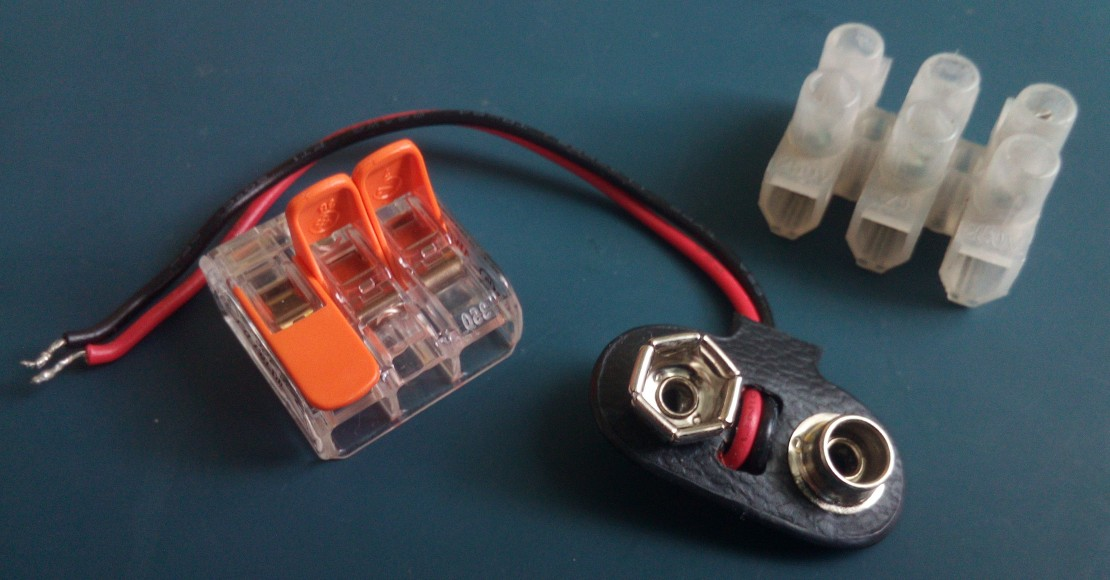
\includegraphics[height=3.3cm]{zasilanie}\end{center}

Jeżeli po zakończeniu kursu będziesz chiał(a) kontynuować zabawę z elektroniką warto pomyśleć o zakupie jakiegoś źródła zasilania z regulacją napięcia i ograniczenia prądowego.
Na przykład w postaci przetwornicy DC-DC z regulacją tych parameterów i wyświetlaczem pokazującym wartość napięcia oraz zasilacza wtyczkowego 12V DC.

\subsection{Podzespoły elektroniczne}

Będzie potrzebny też zestaw drobnych podzespołów elektronicznych:
\begin{itemize}
	\item rezystory 1kΩ i 22kΩ, po około 10 sztuk
	\item potencjometr / rezystor nastwany 5kΩ, który da się włożyć w płytkę stykową, najlepiej wieloobrotowy, 1-2 sztuki
	\item kondensator elektrolityczny 100uF, kilka sztuk
	
	\item dioda prostownicza, około 10 sztuk
	\item dioda świecąca, około 10 sztuk
	\item dioda Zenera 3.3V, około 5 sztuk
	\item tranzystor NPN (np. BC337) i PNP (np. BC327), po kilka sztuk
	
	\item układ logiczny z serii 4000\footnotemark[2]: NAND (np. CD4011BE) lub NOR (np. CD4001BP)
	\item rejestr przesuwny z serii 4000\footnotemark[2] (np. CD4094B)
	\item rejestr z interfejsem I2C\footnotemark[3] (np. PCF8574A lub MCP23008)
\end{itemize}

\footnotetext[2]{Jeżeli kupujesz inne zbliżone układy zwróć uwagę aby w zakresie rekomendowanego napięcia zasilania znajdowało się zarówno 3.3V jak i 9V.}
\footnotetext[3]{Tutaj nie musisz szukać układów akceptujących 9V napięcia zasilania, wystarczy praca dla 3.3V i 5V.}

\input{booklets-sections/warsztat/16-zakupy-inne.tex}

\copyrightFooter{
	© Matematyka dla Ciekawych Świata, 2021.\\
	© Robert Ryszard Paciorek <rrp@opcode.eu.org>, 2021.\\
	Kopiowanie, modyfikowanie i redystrybucja dozwolone pod warunkiem zachowania informacji o autorach.
}
\end{document}
